\documentclass[../document.tex]{subfiles}
\begin{document}
\section{Model}
This section gives an high level overview of the steps in our approach. We will first describe the data gathering,  then the post processing pipeline used to generate the dataset. After, we will introduced the model used to fit the data and then show the results with different test environments.
\subsection{Robot: Krock}
Our task was to apply the approach proposed in \cite{omar@traversability} with a legged robot developed at EPFL named 
\emph{Krock}. Figure \ref{fig:krock} shows the robot in the simulated environment.
\begin{figure}[H]
    \centering
    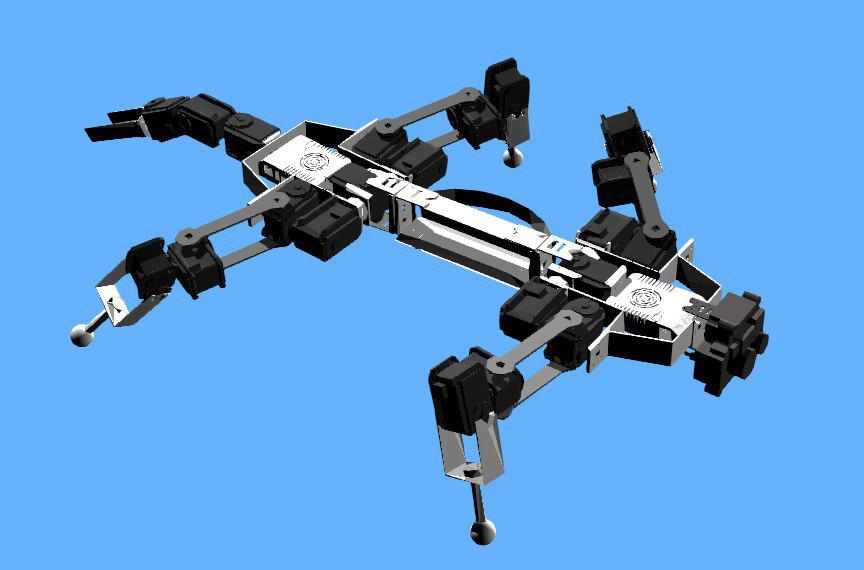
\includegraphics[width=\linewidth]{img/krock-1.jpg}
    \label{fig:krock}
    \caption{\emph{Krock}}
\end{figure}
Krock has four legs, each one of them is equipped with three motors in order to rotate in each axis. The robot is 
also able to rise itself in three different configurations, gait, using the four motors on the body connected 
to the legs. In addition, there are an other set of two motors in the inner body part to increase krock's move set. 
The tail is composed by another set of three motors and can be used to perform a wide array of tasks.
The robot is $85cm$ long and weights around $1.4kg$. The next figure \ref{fig:krock-top} shows \emph{Krock} from the top helping the reader understanding its composition and the correct ratio between its parts. Figure ]\ref{fig:krock-top-details} shows krock's dimensions in centimeters and highlight each motor with a red marker/
\begin{figure}[H]
    \centering
    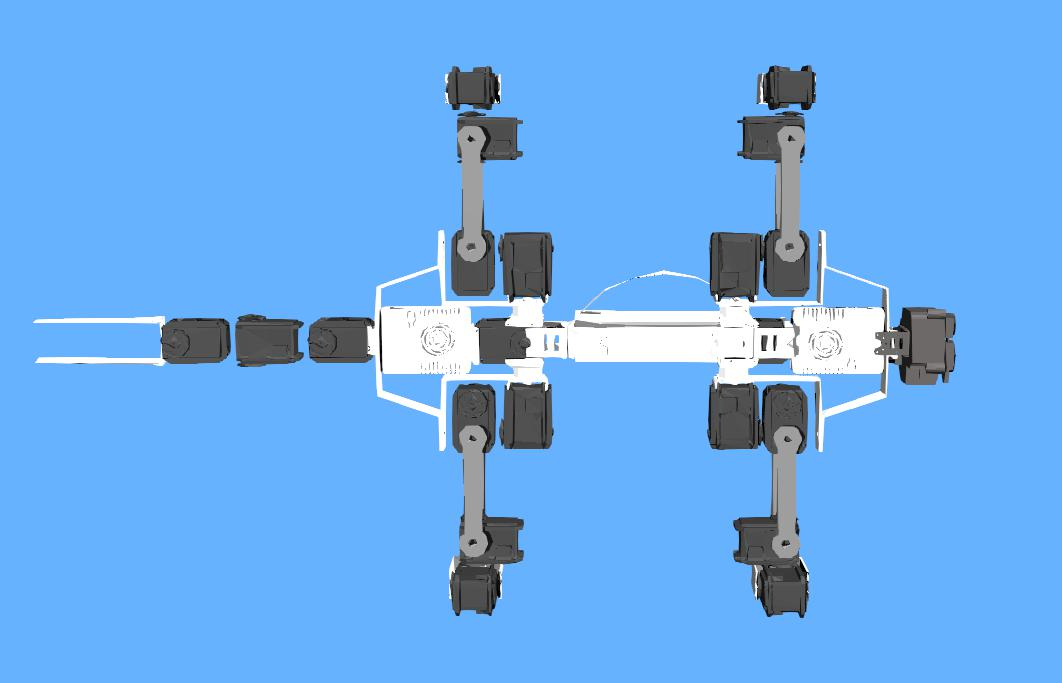
\includegraphics[width=\textwidth]{img/krock-top.jpg}
    \label{fig:krock-top}
    \caption{Top view of \emph{Krock}}
\end{figure}
\begin{figure}[H]
    \centering
      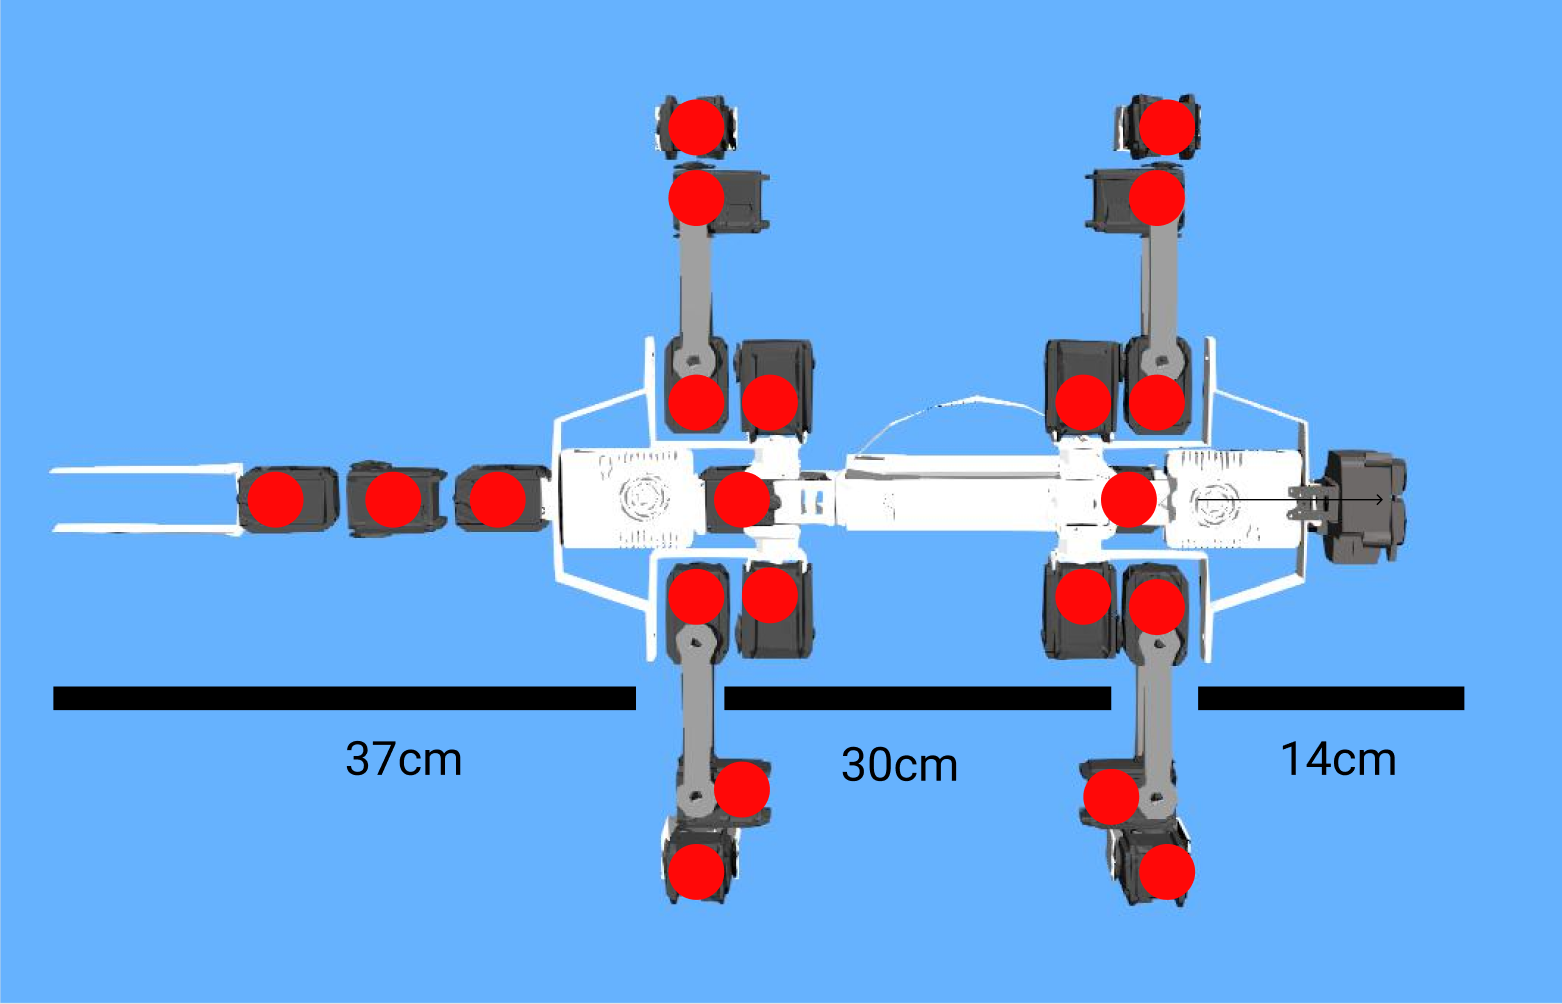
\includegraphics[width=\textwidth]{img/krock-top-highlight.png}
    \label{fig:krock-top-details}
    \caption{Details highlighted in \emph{Krock}}
\end{figure}
\emph{Krock}'s moves by lifting and moving forward one leg after the other. The following figure shows the robots going forward.
	\begin{figure}[H]
    	\begin{subfigure}[b]{0.3\textwidth}
			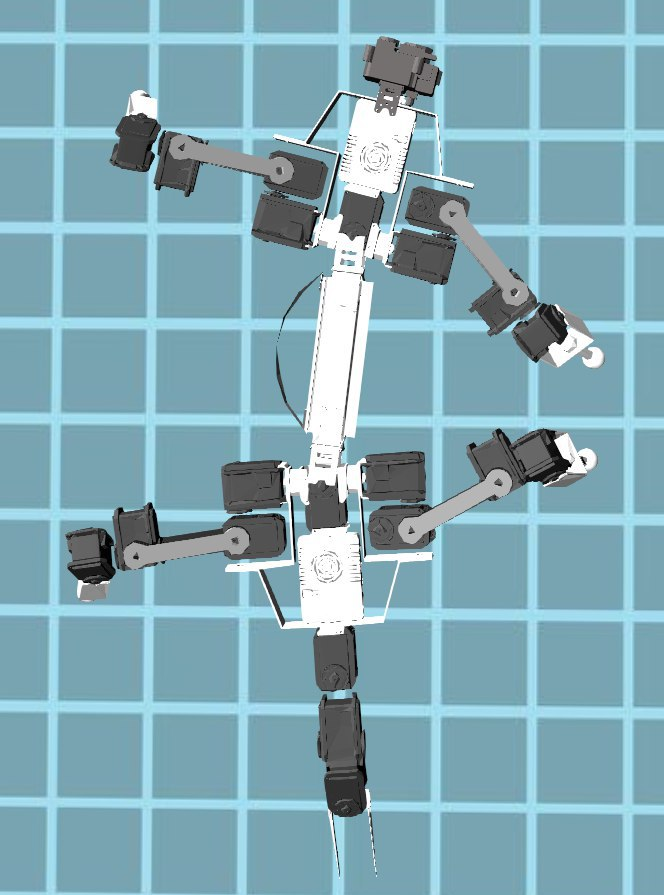
\includegraphics[width=\textwidth]{img/krock-moving-1}
			\caption{$t=1$}
	    \end{subfigure}
		\begin{subfigure}[b]{0.3\textwidth}
			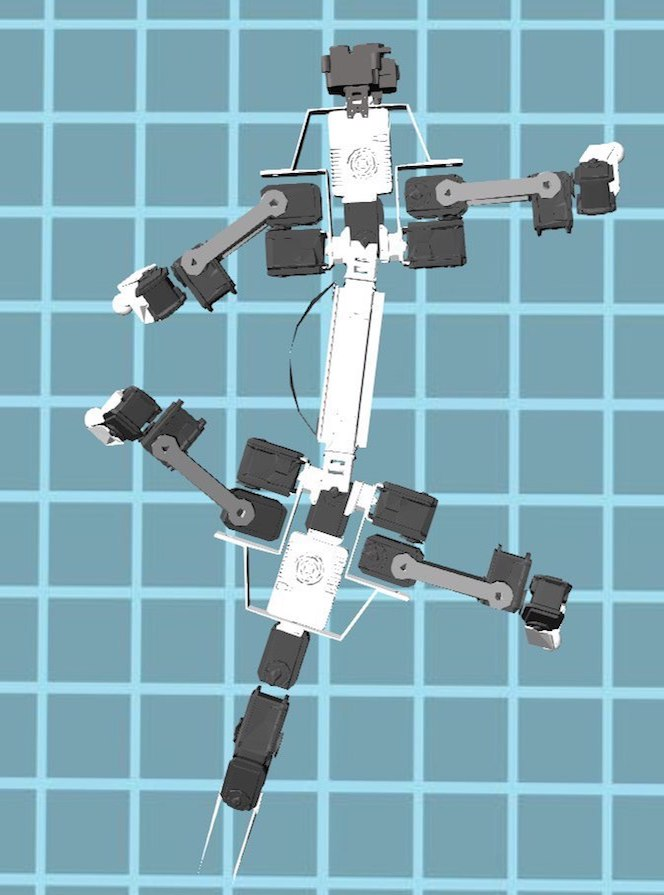
\includegraphics[width=\textwidth]{img/krock-moving-2}
			\caption{$t=2$}
	    \end{subfigure}	
	   \begin{subfigure}[b]{0.3\textwidth}
			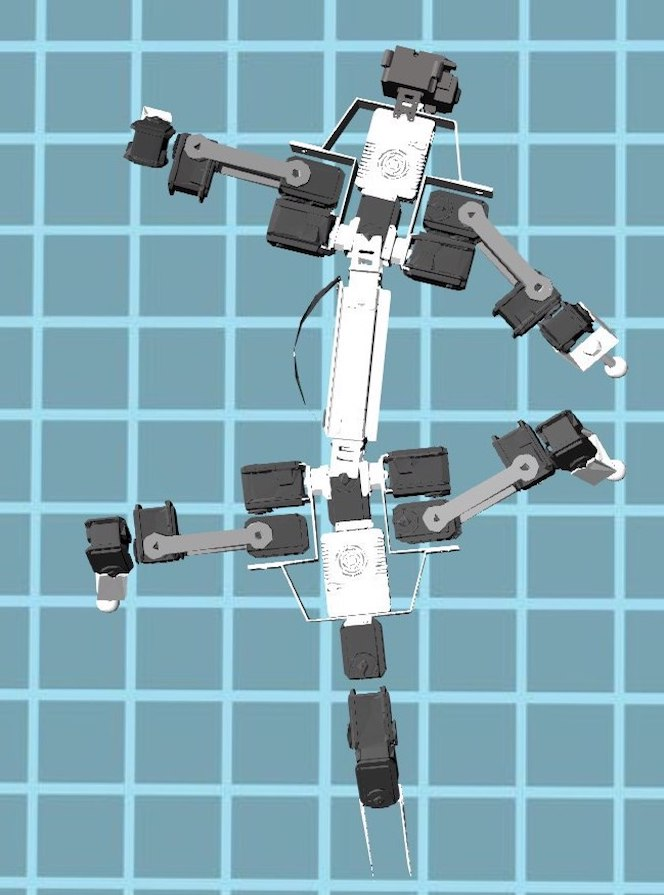
\includegraphics[width=\textwidth]{img/krock-moving-3}
			\caption{$t=3$}
	    \end{subfigure}	
	\label{fig: krock-moving}
	\caption{\emph{Krock} moving forward.}
	\end{figure}
\emph{Krock} can also raise its own body in three different configurations. Figure 

\todo[inline]{Add Krock gait picture}

\begin{figure}
\ref{fig: krock-gait}
\caption{\emph{Krock} differents gait configuration.}	
\end{figure}
\subsection{Simulation}
Our approach relies on simulations to collected the data needed to train the estimator. We used Webots \cite{webots}, a professional 
mobile robot simulator, as backbone for our framework. 

We generate fifteen synthetic $10x10$ meters long heightmaps with different features, such as walls, bumps and slopes using the same techniques described in \cite{omar2018traversability}. Figure \ref{fig:heightmaps}
show some of the maps used in the simulator. 

A heightmap is grey image, formally a 2D array, where each element, pixel, represents a height value. Since each image has a range from $[0,255]$, we also need to scale them when needed. For this reason, we associated a height scaling value for each heightmap that is used to increase or decrease the steepness. 

\todo[inline]{Add heightmap picture}
\todo[inline]{Add heightmap and a 3d render of that map}
\todo[inline]{add two 3d render of a map with two different height values}

\begin{figure}[H]
    \todo[inline]{TODO}
\label{fig:heightmaps}
\caption{Some of the heightmaps used in the simulation.}
\end{figure}

To generate the train data, each map is loaded into the simulator, then the robot is spawned in the world and we let it walked forward for a certain amount of time or until it reaches the edge of the map. While moving, we store his pose, that contains position and orientation, with a rate of $50hz$. 

We run fifteen simulations, one simulation is defined as one robot spawns and death, for each map with a height scale factor of one. We also decide to include steepest training samples by using one of the maps with a slope with heights factors from $[1,7]$. The following pictures shows this specific map with different scaling factors. 

\todo[inline]{add slope map with different height values}

\emph{Krock} is equipped with a controller implemented using the Robotic Operating System (ROS) that is used as a communication channel between our framework and the simulator. Basically, ROS exposes nodes, called \emph{topics}, in which we can listen for incoming messages. Thus, \emph{Krock} is able to stream its pose to all the clients connected to its pose topic. 

We also generate the test set, by running the robot in real world environment, such as \emph{Quarry} a cave map, that we later use to test the fitted model. 

\todo[inline]{Add the querry 3d height map / 3d render)



\end{document}
